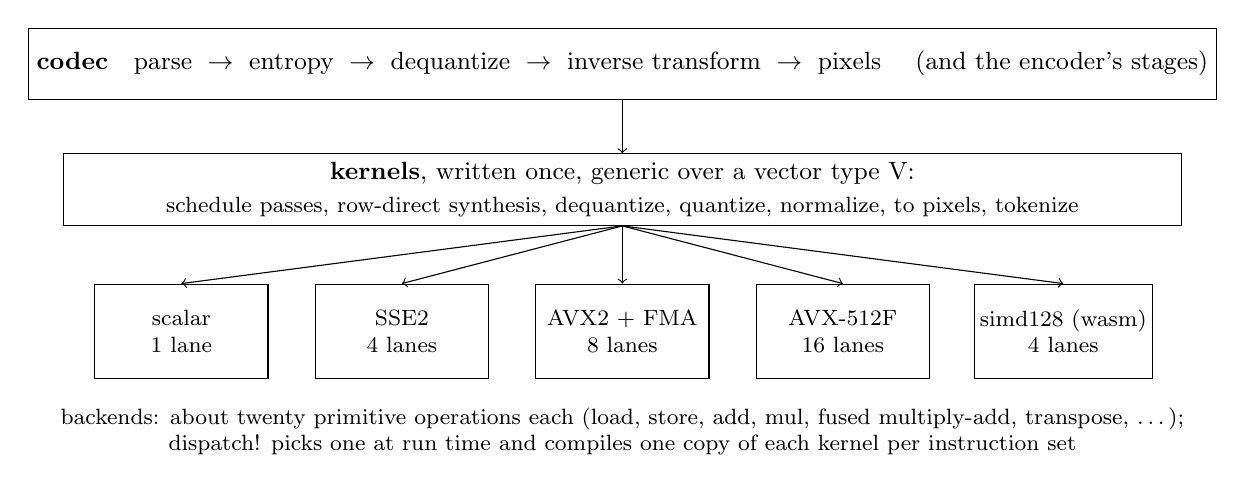
\begin{tikzpicture}[font=\small,
    layer/.style={draw,minimum height=9mm,align=center,inner sep=3pt},
    be/.style={draw,minimum height=12mm,minimum width=22mm,align=center,inner sep=2pt,font=\footnotesize}]
  % codec stages
  \node[layer,minimum width=14.2cm] (codec) at (0,3.2)
    {\textbf{codec}\quad parse \;$\to$\; entropy \;$\to$\; dequantize \;$\to$\; inverse transform \;$\to$\; pixels
     \quad(and the encoder's stages)};
  % kernels
  \node[layer,minimum width=14.2cm] (kern) at (0,1.6)
    {\textbf{kernels}, written once, generic over a vector type \code{V}:\\[1pt]
     \footnotesize schedule passes, row-direct synthesis, dequantize, quantize, normalize, to pixels, tokenize};
  % backends
  \node[be] (s) at (-5.6,-0.2) {scalar\\1 lane};
  \node[be] (sse) at (-2.8,-0.2) {SSE2\\4 lanes};
  \node[be] (avx) at (0,-0.2) {AVX2 + FMA\\8 lanes};
  \node[be] (avx5) at (2.8,-0.2) {AVX-512F\\16 lanes};
  \node[be] (w) at (5.6,-0.2) {simd128 (wasm)\\4 lanes};
  \node[font=\footnotesize,align=center,anchor=north] at (0,-1.05)
    {backends: about twenty primitive operations each (load, store, add, mul, fused multiply-add, transpose, \dots);\\
     \code{dispatch!} picks one at run time and compiles one copy of each kernel per instruction set};
  \draw[->] (codec) -- (kern);
  \foreach \b in {s,sse,avx,avx5,w} \draw[->] (kern.south) -- (\b.north);
\end{tikzpicture}
